
\documentclass{article}
\usepackage{graphicx}
\begin{document}
\title{Hidden Markov model}


\author{Sachin Malve \\
	19111049 \\
 	5th Semester \\ 
	Biomedical Engineering\\
	}

\maketitle 
 \hrulefill

\section{Introduction}
A Markov chain or Markov process is a stochastic model describing a sequence of possible events in which the probability of each event depends only on the state attained in the previous event. And Hidden Markov Model (HMM) is a statistical Markov model in which the system being modeled is assumed to be a Markov process with unobserved (i.e. hidden) states.Hidden Markov Models are widely used for reinforcement learning, temporal pattern recognition such as speech, handwriting, gesture recognition, part-of-speech tagging, musical score following, partial discharges and bioinformatics.

\section{Intuition behind HMMs}
HMMs are probabilistic models. They allow us to compute the joint probability of a set of hidden states given a set of observed states. The hidden states are also referred to as latent states. And after we know the joint probability of hidden variables we use it to find the highest probability and select it is as hidden state.
\\
There are 3 types of states :-
\\
Transition Data - Probability of transitioning to a new state conditioned on a present state.
\\
Emission data — Probability of transitioning to an observed state conditioned on a hidden state.
\\
Initial state information — Initial probability of transitioning to a hidden state. This can also be looked at as the prior probability. 

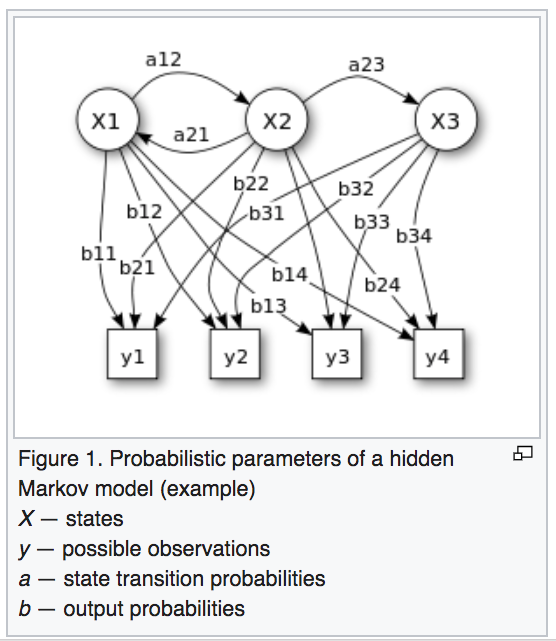
\includegraphics[scale=.50]{0_s4wQ8nTIb2122-9s} 

\section{Assumptions in HMM}
Hidden Markov Models have a few assumptions.
\\
Output independence assumption: Output observation is conditionally independent of all other hidden states and all other observations when given the current hidden state.
\\
Emission Probability Matrix 

\section{Application of HMM}
They are widely used,In health care field such as DNA Sequence Analysis,Protein Family Profiling, Prediction of Genes, Radiation Hybrid Mapping,Prediction of DNA Functional Sites,Horizontal gene Transfer.
\\
And in other areas like Speech recognition, gesture recognition,Language Modeling,Stock price  prediction too. 


\end{document}